\chapter{Partitioning Space}%DCG "The S-System" Sec.9, p85
    \label{sec:fine}
    \oldlabel{2}

\section{Interaction of $V$-cells with the $Q$-system}

We study the structure of one $V$-cell, which we take to be the
$V$-cell at the origin $v=0$.  Let $\CalQ$ be the set of simplices
in the $Q$-system.  For $v\in\Lambda$, let $\CalQ_v$ be the subset
of those with a vertex at $v$.\index{Qv@$\CalQ_v$}



\begin{lemma} \label{lemma:voronoi-truncation-over-Q}
If $x$ lies in the \index{Voronoi cell} Voronoi cell at the
origin, but not in the $V$-cell at the origin, then there exists a
simplex $Q\in\CalQ_0$, such that $x$ lies in the cone (at $0$)
over $Q$. Moreover, $x$ does not lie in the interior of $Q$.
\end{lemma}

\begin{proof}
By
the definition of $V$-cell, there is a barrier $\{v_1,v_2,v_3\}$
that meets $\op{conv}^0(0,x)$.  
By Lemma~\ref{tarski:vor-bar-tet}
and Lemma~\ref{tarski:vor-bar-quad},
the simplex $Q=\{0,v_1,v_2,v_3\}$ is a quasi-regular tetrahedron
or a flat quarter.  If it is a flat quarter then it shares a diagonal
with a barrier coming from the $Q$-system.  Thus, $Q$ is in
the $Q$-system too.  By Lemma~\ref{tarski:pass-cone}, the
point $x$ lies in the cone over $Q$.

If $x\in\op{conv}^0(Q)$, then the barrier, which is a face
of $Q$, does not separate
$x$ from $v$.  The rest is clear.
\end{proof}



\begin{lemma}\label{lemma:VC-Omega}
Inside the ball of radius $t_0$ at the origin, the $V$-cell and
Voronoi cell coincide:
   $$B(0,t_0)\cap \op{VC}(0) \equiv B(0,t_0)\cap \Omega(0).$$
That is, they are equal up to a null set.
\end{lemma}

\begin{proof} Let $x\in B(0,t_0)\cap \op{VC}(0)\cap\Omega(v)$, where
$v\ne0$.  
% By Lemma~\ref{lemma:unobstr-t0}, 
The origin is
unobstructed\tarf{FFSXOWD} at $x$.  Thus, $|x-v|< |x|\le t_0$.  By
Lemma~\ref{lemma:unobstr-t0} again, $v$ is unobstructed at $x$, so
that $x\in \op{VC}(v)$, contrary to the assumption
$x\in\op{VC}(0)$.  Thus $B(0,t_0)\cap\op{VC}(0)\subset\Omega(0)$.
Similarly, if $x\in B(0,t_0)\cap \Omega(0)$, then $x$ is
unobstructed at the origin, and $x\in \op{VC}(0)$.
\end{proof}

\bigskip

\begin{remark} The next lemma helps to determine which $V$-cell
a given point $x$ belongs to.  If $x$ lies in the open cone over a
simplex $Q_0$ in $\CalQ$, then Lemma~\ref{lemma:Q-divide}
describes the $V$-cell decomposition inside $Q$;  beyond $Q$ the
origin is obstructed by a face of $Q$, so that such $x$ do not lie
in the $V$-cell at $0$. If $x$ does not lie in the open cone over
a simplex in $\CalQ$, but lies in the open cone over a standard
region $R$, then Lemma~\ref{lemma:V-cell-local} describes the
$V$-cell.  It states in particular, that for unobstructed $x$, it
can be determined whether $x$ belongs to the $V$-cell at the
origin by considering only the vertices $w$ that lie in the closed
cone over $R$ (the standard region containing the radial
projection of $x$). In this sense, the intersection of a $V$-cell
with the open cone over $R$ is {\it local\/} to the cone over $R$.
\end{remark}



Let $\CalB_0'$ be the set of triangles $T$ such that at least one
of the following holds:
\begin{itemize}
    \item $T$ is a barrier at the origin, or
    \item $T=\{0,v,w\}$ consists of a diagonal of a quarter in the
    $Q$-system together with one of its anchors.
\end{itemize}

%DCG Lemma 5.29, page 50.
\begin{lemma} [Decoupling Lemma]\label{lemma:V-cell-local}
%Let $x\in I_0$, the cube of side $4$ centered at the origin
%parallel to coordinate axes.  
Assume that the closed segment
$\{x,w\}$ intersects the closed $2$-dimensional cone with center
$0$ over $F=\{0,v_1,v_2\}$, where $F\in\CalB'_0$. Assume that the
origin is not obstructed at $x$. Assume that $x$ is closer to the
origin than to both $v_1$ and $v_2$. Then $x\not\in\op{VC}(w)$.
\end{lemma}
\index{decoupling lemma}

\begin{remark}  The Decoupling Lemma is a crucial result.  It
permits estimates of the scoring function in
\Chap~\ref{sec:scoring} to be made separately for each standard
region.  The estimates for separate standard regions are far
easier to come by than estimates for the score of the full
centered packing.  Eventually, the separate estimates for each
standard will be reassembled with linear programming techniques in
\Chap~\ref{sec:linearprogram}.
\end{remark}

\begin{proof}
Assume for a contradiction that $x$ lies in $\op{VC}(w)$. In
particular, we assume that $w$ is not obstructed at $x$.  Since
the origin is not obstructed at $x$, $w$ must be closer to $x$
than $x$ is to the origin.

By Lemma~\ref{tarski:decouple}, 
   $|w|,|w-v_1|,|w-v_2|\le 2t_0$.  Thus, $Q=\{0,w,v_1,v_2\}$ is
a quarter or a quasi-regular tetrahedron.  By the definition of
$\CalB'_0$, the face $F$ must lie in the $Q$-system.  Thus,
$F$ is a barrier.  Again, by Lemma~\ref{tarski:decouple},
$\op{conv}(F)$ meets the segment from $x$ to $w$, so $x$ is obstructed
at $w$.  Thus, $x$ does not lie in $\op{VC}(w)$.
\end{proof}

%\section{Local Optimality}%DCG Sec. 8, p72  
%\label{sec:local-opt}
%Moved after the main estimate.




\section{Overview}%DCG 9.1, p95
    \label{sec:fine-overview}
    \oldlabel{2.1}



In this \chap, we define a decomposition of a $V$-cell. Let
$\op{VC}$ be the $V$-cell at the origin.  For any $t > 0$, let
$V(t)$ be the intersection of $\op{VC}$ with the ball $B(0,t)$ at
the origin of radius $t$. We write $\op{VC}$ as the disjoint union
of $V(t_0)$ and its complement $\delta$.

Assume that there is an upright 
diagonal $\{0,v\}$. 
We will define $\delta_i(v)\subset\delta$, where $i$ runs
over some finite indexing set.
The sets $\delta_i(v)$ will be defined so as not to overlap
one another. 

We will define a set $\CalS$ of simplices, each having a vertex at
the origin. (The letter `$\CalS$' is for simplex.)
The vertices of the simplices will be vertices of the
packing, and their edges will have length at most $2\sqrt{2}$. The
sets $\op{cone}^0(0,S)$, for distinct $S\in\CalS$, will not overlap. Over a
simplex $S\in\CalS$, the $V$-cell will be truncated at a radius
$t_S\ge t_0$. After defining the constants $t_S$, we will set
    $$V_S(t_S) = \op{cone}^0(0,S) \cap V(t_S) =\op{cone}^0(S)\cap B(t_S)\cap \op{VC}(0).$$
That is, $V_S(t_S)$ is the part of the $V$-cell at the origin,
contained in the cone over $S$ and in the ball of radius $t_S$.
If
    $\op{VC}(0) \cap \op{cone}^0(S)\subset B(t_S)\subset B(t'_S)$,
then
    $V_S(t_S)=V_S(t'_S)$.

Since $t_S\ge t_0$, the sets $V_S(t_S)$ and $\delta$ may meet at
interior points. Nevertheless, we will show that $V_S(t_S)$ does
not meet the interior of any $\delta(v)$.  Let $\tildeV(t_0)$ be
the set of points in $V(t_0)$ that do not lie in $\op{cone}^0(S)$,
$S\in\CalS$. We will derive an explicit formula for the volume of
$\tildeV(t_0)$.

In $\op{VC}(0)$, there are nonoverlapping sets
$$\delta(v),\quad   V_S(t_S),\quad \tildeV(t_0).$$
Let $\delta'$ be the complement in $\op{VC}(0)$ of the union of
these sets. These sets give a decomposition of $\op{VC}(0)$.
Corresponding to this decomposition is a formula for $\sigma(D)$
of the form
    $$
    \sigma(D) =
        \op{c-vor}(\tildeV(t_0))
        + \sum_{\CalS}\op{c-vor}(V_S(t_S))
        -\sum_{v,i} 4\doct\op{vol}(\delta_i(v))
        -4\doct\op{vol}(\delta').
    $$
Since $\op{vol}(\delta')\ge0$, we obtain an upper bound on
$\sigma(D)$ by dropping the rightmost term.



\section{The set $\delta(v)$}%DCG 9.2, p86
    \label{sec:deltaP}
    \oldlabel{2.3}



\begin{definition}\label{def:eta0}
Set $\eta_0(h)=\eta(2h,2,2t_0)$.
\index{zzeta@$\eta_0$}
\end{definition}

%By Lemma~\ref{tarski:1453}, 
%if $h\le\sqrt2$, then $\eta_0(h)\le \eta_0(\sqrt2) <
%1.453$.\index{ZZZZ1.453@1.453}



Let $v$ be a vertex with $2t_0 < |v| <\sqrt8$.
Let $D_0 = \op{rcone}^0(0,v,|v|/(2\eta_0(|v|/2)))$.
Let $v_1,\ldots,v_k$ be the anchors around $\{0,v\}$ indexed
cyclically. The half planes $A_i=\op{aff}_+(\{0,v\},v_i)$
slice $\ring{R}^3$ into $k$ open wedges
$W_i$, between
    $A_i$ and $A_j$,
where $j\equiv i+1\mod k$, so that
    $D\ring{R}^3\setminus (A_1\cup\cdots\cup A_k) =\cup W_i$.

\begin{definition}\label{def:wedge}
Let $\CalW=\CalW(0,v)$ be the set of wedges $W=W_i$ along $(0,v)$ 
such that either
\begin{enumerate}
    \item The azimuth angle of $W$ (along $\{0,v\}$) is at least $\pi$.
    \item The azimuth angle of $W$ is less than $\pi$, 
 $|v_i-v_j|\ge 2.77$,
    $\rad(0,v,v_i,v_j)\ge\eta_0(|v|/2)$, and the
    circumradius of $\{0,v_i,v_j\}$ or $\{v,v_i,v_j\}$ is
    $\ge\sqrt2$.
    \label{enum:wedge2}
\end{enumerate}
\index{wedge}
\index{W@$\CalW$}
\end{definition}

(If $(0,v)$ has only one or two anchors, then it is understood
 that $W$ is all of $\ring{R}^3$ or all of $\ring{R}^3$, except a half-plane.)
Fix $i,j$, with $j\equiv i+1\mod k$. If $W = W_i$ is a wedge in
$\CalW$, let $\{0,v_i,v\}^\perp$ be the plane through the origin and
the circumcenter of $\{0,v_i,v\}$, perpendicular to $\{0,v_i,v\}$.
Skip the following step if the circumradius of $\{0,v_i,v\}$ is
greater than $\eta_0(|v|/2)$, but if the circumradius is at most
this bound, the plane
of $\{0,v_i,v\}^\perp$
intersects the right circular cone boundary of $D_0$ along two rays
emanating from $0$.  Let $c_i$ be a point on the ray (selected on
the $W$-side of $\{0,v_i,v\}$).  Simlarly, we construct the point
$c_i'$ for $\{0,v,v_j\}$ (again on the $W$-side).

Define $\theta=\theta(v)$ by $\cos\theta = |v|/(2\eta_0(|v|/2))$.
If Condition~2 holds, we let $c$ be the 
circumcenter of $\{0,v_i,v_j,v\}$.  The angle
at $0$ between $c$ and $v$ is
$\theta'$, where
$$\cos\theta' = |v|/(2\rad)\le |v|/(2\eta_0) = \cos\theta.$$
We conclude that $\theta'\ge\theta$ and $c$ does not lie in $D_0$.
Thus, the half-planes
   $$
   A_i,\quad B_i=\op{aff}_+(\{0,v\},c_i),\quad 
   B'_i = \op{aff}_+(\{0,v\},c'_i), \quad
   A_j
   $$
are ordered cyclically around $\{0,v\}$. (Set $B_i=A_i$
or $B'_i=A_j$, if the corresponding circumradius is greater than
$\eta_0(|v|/2)$.)
Let $W'=W'_i$ be the open wedge of $D_0$ between $B_i$ and $B'_i$.
Let
    $$E_w = \{x : 2 x\cdot w \le w\cdot w\},$$
for $w = v,v_i,v_j$. These are half-spaces bounding the Voronoi
cell. Set $E_\ell = E_{v_\ell}$.

\begin{definition} \label{def:delta-e}
In both cases (Conditions~1 and~2), let $W$ be the wedge between
$v_i$ and $v_j$ along $(0,v)$, $W'$ the smaller wedge, 
and let $c=\eta_0(|v|/2)$ in
    $$
    \begin{array}{lll}
      \BigD'(v,W) &= [E_v\cap W'\cap D_0]\cup \op{rog}^0(0,v,v_i,p_i,c)
      \cup \op{rog}^0(0,v,v_j,p_j,c)
      \\
    \BigD(v,W) &= \BigD'(v,W) \cup 
    \op{rog}^0(0,v_i,v,p_i,c)
    \cup \op{rog}^0(0,v_j,v,p_j,c)\\
    \bigd(v,W) &= \{x\in\BigD(v,W)\mid |x|>t_0\},
    \end{array}
    $$
where $p_i,p_j$ are selected so that the simplices $\op{rog}^0$ lie
in the wedge $W$.
\index{zzdelta@$\bigd(v,W)$}
\index{zzDelta@$\BigD(v,W)$}
\end{definition}

\begin{remark} We note that the union is actually a disjoint union,
and that each of the pieces is one of the primitive regions, so
the volume of $\BigD$ is immediate.
\end{remark}

\begin{figure}[htb]
  \centering
  \includegraphics{\ps/diag46.ps}
  \caption{$\BigD(v,W)$ lies in a cone. The intersection of
    that cone with the unit sphere is the shaded region.}
  \label{fig:anchor-quarter}
\end{figure}

\begin{remark}
Recall that in the definition of Rogers simplex (Definition~\ref{def:rog}, 
it is defined to be the
empty set 
if the corresponding parameters are not coherent.  It is to
be understood that the all discussion regarding this set
can (and should) be disregarded in the case that it is empty.
\end{remark}

We present a series of lemmas that explore the geometry of the sets
$\BigD(v,W)$.



\begin{lemma}\label{lemma:new-anchor}
  Let $S=\{0,v,w,u\}$ be a simplex.  Assume that $\{0,v\}$ is an
upright diagonal, that $w$ and $u$
are anchors of $\{0,v\}$, and that $\rad(S)< \eta_0(|v|/2)$.
Assume there is a wedge $W$ of $\CalW$ along the face $\{0,v,w\}$
(on the same side of the face as $u$).  
Then there exists an anchor $w'$ of $\{0,v\}$ between $u$ and $w$
(that is, in $\op{aff}_+^0(\{0,v\},\{u,w\})$) with
    $|w'-w|\ge2.77$ and
    $\rad\{0,w,w',v\} \ge \eta_0(|v|/2)$.
\end{lemma}

\begin{proof} The conditions on $S$ are incompatible with the
conditions of Definition~\ref{def:wedge} defining wedges.
Therefore, $w$ and $u$ cannot be consecutive anchors around
$\{0,v\}$.  Let $w'$ be the anchor such that $S'=\{0,v,w,w'\}$
determine the wedge $W$.  Since $w$ and $w'$ are consecutive anchors,
we see that $w'$ must be between $u$ and $w$.  It must have the
second type in Definition~\ref{def:wedge}.  The conclusion follows.
\end{proof}






In the following lemmas, we adopt a uniform notation.
$\{0,v\}$ is always be an upright diagonal: $|v|<\sqrt8$.
$W$ is  a wedge along $(0,v)$
between two anchors $w$ and $w'$.  Set $R_w=\op{rog}^0(0,w,v,p,\eta_0(|v|/2))$,
where $p$ is selected so that $R_w$ lies in $W$.


The following definition will be used briefly, then discarded.
Its purpose is to group together a few separate cases in the next
few lemmas.

\begin{definition}  Let $(0,v,u_1,u_2)$ be a four-tuple of vertices
in $\ring{R}^3$.  We say that it is {\it normal} if $2t_0<|v|<\sqrt8$
and one of the
following holds:
\begin{enumerate}
  \item (qrt) $\{0,u_1,u_2\}$ is a quasi-regular triangle.
  \item (upright) $\{0,u_1,u_2\}$ is an upright triangle; that is, say,
    $2t_0 < |u_1| < \sqrt8$, and $u_2$ is an anchor of $u_1$.
  \item (flat)
   $2t_0<|u_1-u_2|<\sqrt8$; and if $u_1,u_2$ are both anchors $(0,v)$, 
   then
    no further anchor of $\{0,v\}$
   lies in the lune $\op{aff}^0_+(\{0,v\},\{u_1,u_2\})$.
\end{enumerate}
\end{definition}

\begin{lemma}\label{lemma:BigD-}  Let $S=(0,v,u_1,u_2)$ be normal.
Then
$\BigD'(v,W)$ does not meet $F=\op{cone}(0,\{u_1,u_2\})$.
\end{lemma}

\begin{proof}  By elementary geometry\tarf{tarski:eps-bigd-}, 
the hypotheses imply
that $S$ is normal of the flat or qrt variety, and 
that $u_1$ and $u_2$ are anchors.  The lemma also
gives that 
$\rad(S)<\eta_0(|v|/2)$.    
In the qrt case, $S$ forms
an upright quarter.  By elementary geometry\tarf{tarski:consec-anchors}, $u_1$ and $u_2$
are consecutive anchors. In the flat case as well, 
$u_1$ and $u_2$ are consective
anchors around $\{0,v\}$.

If the wedge $W$ is not between
the anchors $u_1$ and $u_2$, then $\BigD$ lies outside the 
lune $\op{aff}_+^0(\{0,v_0\},\{u_1,u_2\})$, but $F$ lies inside it.  Thus,
the wedge must run between $u_1$ and $u_2$.   This contradicts 
the rules for forming wedges.  (See
Lemma~\ref{lemma:new-anchor}, which implies that
anchors $u_1$ and $u_2$ cannot be consecutive.)
\end{proof}

\begin{lemma}\label{lemma:fine-Rw}
Let $S=(0,v,w,u_1)$ be normal.
Suppose that $w$ is an anchor of $\{0,v\}$.
Then
$R_w$
does not meet $F=\op{cone}(0,\{u_1,u_2\})$.
\end{lemma}

\begin{proof}  We can use the same proof as in Lemma~\ref{lemma:BigD-},
except with one lemma\tarf{tarski:eps:fine:Rw} substituted for 
another\tarf{tarski:eps-bigd-}.
\end{proof}

\begin{lemma}\label{lemma:fine:barrier}  
Let $S=\{0,v,w,u\}$ be a set of four distinct vertices
in the packing.  Assume that $\{0,v\}$ is an upright diagonal of
a quarter in the $Q$-system and that $w$ is an anchor of $\{0,v\}$.
Let $R_w$ be as above; that is, a Rogers simplex attached to a wedge
$W\in \CalW$ around the diagonal $\{0,v\}$.
Assume $x\in R_w$ satisfies $\epsilon_0(x,\{v,w,u\})= u$.
Then there exists a vertex $w'$ that is an anchor of $\{0,v\}$ such
$b=\{v,w',0\}$ is a barrier and $x$ is obstructed from $u$
by $b$.
\end{lemma}

\begin{proof} Assume for a contradiction that $\epsilon_0(x)=u$.
We separate the proof into two cases, depending on whether
$x$ and $u$ lie on the same side of $A=\op{aff}(v,w,0)$.

Assume that $x$ and $u$ lie on opposite sides of $A$.
For any nonzero vertices $v',v''$,
Let $L(v',v'')$ be the line of points equidistant from $\{0,v',v''\}$.
The three lines $L(u,v)$, $L(v,w)$, $L(u,w)$ meet at the circumcenter
$c$ of $S$.  The rays $L^+(u,v)$, $L^+(v,w)$, $L^+(u,w)$ demarcate
the regions between $\epsilon_0=w,u,v$.  (Pick the direction
of ray so that it runs through the circumcenter of the face $\{0,v',v''\}$
if the remaining vertex has positive orientation, and so that it
runs in the opposite direction otherwise.)

If $u$ has positive orientation in $S$, then $L^+(v,w)$ runs through
the circumcenter of $\{0,v,w\}$ and along an edge of $R_w$.
The point $w/2$ in the closure of  $R_w$ also has $\epsilon_0=w$.
It follows that $\epsilon_0$ has value $w$ on $R_w$, which is contrary
to our assumption.

Thus, $u$ has negative orientation in $S$.  
This implies that $|u-v|,|u-w|,|u|\le 2.51$.  In particular,
$S$ is a quarter.  Since it has the same diagonal as a quarter in
the $Q$-system, we have that $S$ is in the $Q$-system, so that
$\{0,v,w\}$ is a barrier.  By Lemma~\ref{tarski:tip-cone}, we have
that $x\in \op{cone}(u,\{v,w,0\})$.  In particular, $x$ is obstructed
from $u$ by the barrier $\{v,w,0\}$.  Take $w'=w$ in this case.

Now assume that $x$ and $u$ lie on the same side of $A$.
First consider the special case where
we also have that $\rad_V(S)\ge \eta_0(|v|/2)$ and that that
the orientation of $u$ is non-positive in $S$.  In this case, it
follows that $S$ is a quarter in the $Q$-system.  By the rule
for constructing wedges $W\in\CalW$, there is no $R_w$ along $\{0,v,w\}$
in this case.  Next consider the case where
$\rad_V(S)\ge \eta_0(|v|/2)$ and the orientation of $u$ is positive
in $S$.  In this case, the ray $L^+(v,w)$ runs along the edge of 
$R_w$ as before, and we see that $\epsilon_0=w$ on $R_w$.

Finally consider the case where $\rad_V(S)<\eta_0(|v|/2)$.
It follows that $u$ is an anchor of $S$.
By Lemma~\ref{lemma:new-anchor}, there exists a further anchor
$w'$ between $u$ and $w$.  We are in the situation of Lemma~\ref{lemma:prev}.
We have that $\op{conv}\{x,u\}$ meets $\op{conv}\{0,v,w'\}$ and
that $|u-w'|\le 2.51$.  In particular $S'=\{0,v,w',u\}$ is
an upright quarter and $\{0,v,w'\}$ is a barrier.
\end{proof}



\begin{lemma}\label{lemma:fine-Rw:5}
Let $\{0,v,w,u_1,u_2\}$ be a set of five distinct vertices in the
packing.  Assume that $\{0,v\}$ is an upright diagonal of a quarter
in the $Q$-system and that $w$ is an anchor of $\{0,v\}$.
Assume that $S=(0,v,u_1,u_2)$ be normal.
Let $R_w$ be as above; that is, a Rogers simplex attached to a wedge
$W\in \CalW$ around the diagonal $\{0,v\}$.
Then $R_w$ does not meet $F=\op{cone}(0,\{u_1,u_2\})$.
\end{lemma}

\begin{proof}
For a contradiction, assume these sets meet at $x\in R_w\cap F$.
We have $\epsilon_0=\epsilon_0(x,\{w,u_1,u_2\})\in\{w,u_1,u_2\}$.  We consider
two cases depending on whether $\epsilon_0=w$.

Assume that $\epsilon_0=w$.  By Lemma~\ref{tarski:fine:Rw:5},
we have $|w-u_1|\le 2.51$ and $|w-u_2|\le 2.51$.  By the same
lemma, 
there are three possibilities.  The first is that
for either $u=u_1$ or $u=u_2$, we have that $(0,v,w,u)$ is normal
and that $R_w$ meets $\op{cone}(0,\{w,u\})$.  This is contrary to
Lemma~\ref{lemma:fine-Rw:5}.
The second possibility is that
$2.51<|u_1-u_2|<\sqrt8$ and that $v\in\op{cone}^0(0,\{u_1,u_2,w\})$
with $u_1,u_2,w$ all anchors of $\{0,v\}$.  By the normality
hypothesis, these are the only anchors of $\{0,v\}$.  None of the
corresponding wedges $W$ satisfy the conditions to belong to
a wedge of $\CalW$ around $\{0,v\}$.  Thus, this case does not
occur. The third possibility is that $w\in \op{aff}_+(\{0,v\},\{u_1,u_2\})$
and $2.51<|u_1-u_2|$.  This is contrary to the normality
condition on $S$.

In the remaining case, we have $\epsilon_0=u\in\{u_1,u_2\}$.  
Let $S'=\{0,v,w,u\}$.  By Lemma~\ref{lemma:fine:barrier}, there
exist a barrier $b=\{0,v,w'\}$ such that $x$ is obstructed from
$u$ by $b$.  However, if $x\in\op{cone}(0,\{u_1,u_2\})$, then
there exists no such obstruction.  Thus, the intersection
is empty.
\end{proof}

\begin{lemma}\label{lemma:delta-tri}
Let $F=\{0,u_1,u_2\}$ be a quasi-regular triangle.  Let $\{0,v\}$ be
an diagonal. Assume that there
exists a quarter in the $Q$-system along $\{0,v\}$.  Then
$\BigD(v,W)$ does not meet $C=\op{cone}(0,\{u_1,u_2\})$.
\end{lemma}

\begin{proof}
We have separated $\BigD^-(v,W)$ and $R_w$ from $C$.
Together they form $\BigD(v,W)$.
\end{proof}

XX MOve to a section on standard regions.

\begin{corollary}
Each $\BigD(v,W)$ lies entirely in the cone over the standard
region that contains $\{0,v\}$.
\end{corollary}

\begin{proof}
The cone over a standard region is bounded by the cones  over the
quasi-regular triangles.
\end{proof}


\begin{lemma}\label{lemma:delta-flat}
Let $F=\{0,u_1,u_2\}$ be a triangle.  Assume that $|u_1|\le 2t_0$,
$|u_2|\le 2t_0$, and $2t_0\le|u_1-u_2|\le\sqrt8$.  Let $\{0,v\}$
be the diagonal of an upright quarter in the $Q$-system.  Assume
that if $u_1$ and $u_2$ are both anchors of $v$, then they are
consecutive anchors around $v$. Under these conditions, the set
$\BigD(v,W)$ does not overlap the cone at $0$ over the triangle
$F$.
\end{lemma}

\begin{proof} The proof is identical to that of
Lemma~\ref{lemma:delta-tri}. 
\end{proof}

\begin{lemma}\label{lemma:delta-upright}
Let $F=\{0,u_1,u_2\}$ be a triangle.  Assume that $2t_0\le|u_1|\le
\sqrt8$, $2\le|u_2|\le 2t_0$, and $2\le|u_1-u_2|\le2t_0$.  Let
$\{0,v\}$ be the diagonal of an upright quarter in the $Q$-system.
Under these conditions, the set $\BigD(v,W)$ does not overlap
the cone at $0$ over the triangle $F$.
\end{lemma}

\begin{proof}
The proof is identical to that of Lemma~\ref{lemma:delta-tri}.
\end{proof}


\begin{lemma}
Let $\{0,v\}$ be an upright diagonal of a quarter in the
$Q$-system.   If $x$ lies in the interior of $\BigD(v,W)$,
then $x$ is unobstructed at $0$.
\end{lemma}

\begin{proof} For a contradiction, assume that $x$ is obstructed
at $0$ by barrier $T =\{u_1,u_2,u_3\}$.


The convex hull of $T$ can be partitioned into three sets $T(i)$
depending on which vertex of $T$ is closest to a given point in
the convex hull. (Ties can be resolved in any consistent manner.)
Let $y\in \BigD(v,W)$ be the point in the convex hull of $T$ on
the segment from $0$ to $x$.  Fix $i$ so that $y\in T(i)$. If
$v=u_i$, then each point $y$ of $T(i)$ is closer to $v$ than to
$0$.  But each point of $\BigD(v,W)$ is closer to $0$ than to
$v$.  So $x$ is not obstructed by $T$ at $0$.

We may now assume that $v\ne u_i$.

Partition $\ring{R}^3$ geometrically into three sets $V(u_i)$,
$V(0)$, $V(v)$ according to which of $\{u_i,0,v\}$ a point
$z\in\ring{R}^3$ is closest to.  (Again resolve ties in any
consistent manner.)

Assume further that $\max_j u_j \ge 2t_0$. This implies that $y\in
T(i) \subset V(v) \cup V(u_i)$.  On the other hand, we have by
construction that $y\in \BigD(v,W) \subset V(0)$.  (There are
two cases involved in this conclusion, depending on whether $u_i$
is an anchor of $\{0,v\}$.)  However, the sets $V(\cdot)$ are
disjoint; and we reach a contradiction.  Thus, under these
assumptions, $x$ is unobstructed at $0$.

Next assume that $\max_j u_j < 2t_0$.  Let $S=\{0,u_1,u_2,u_3\}$.
Since $T$ is a barrier, $S\in\CalQ_0$.  By assumption, $\{0,v\}$
is a diagonal of an upright quarter in $\CalQ_0$.  By the fact
that the interiors of quarters in $\CalQ_0$ do not meet, we see
that $v$ is not enclosed over $S$.  The set $\BigD(v,W)$ has
a star convexity with respect to the ray from $0$ through $v$.
Thus, if $\BigD(v,W)$ intersects the convex hull of
$T$ at $y$, then $\BigD(v,W)$ intersects the cone over a face
$\{0,u_1,u_2\}$ of $S$ at $y'$. (We can take $y'/|y'|$ to lie on
the cone generated by the arc running from $v/|v|$ to $y/|y|$.
This is impossible by Lemmas~\ref{lemma:delta-tri} and
\ref{lemma:delta-flat}.
\end{proof}

\begin{lemma}  Let $\{0,v\}$ be the upright diagonal of a quarter
in the $\CalQ_0$-system.  Then $\BigD(v,W)$ is
a subset of $\op{VC}(0)$.
\end{lemma}

\begin{proof}
We begin by showing that $\BigD^-(v,W)\subset\op{VC}(0)$.
Suppose to the contrary, that a point $x$ in the interior of
$\BigD^-$ lies in $\op{VC}(w)$, with $w\ne0$.  Then $x$ is closer
to $w$ than to  $0$.  Thus, $\eta(0,v,w)<\eta_0(|v|/2)$, and $w$
is an anchor of $\{0,v\}$.  The face $E_w$ in the construction
$\BigD^-(v,W)$ prevents this from happening.

Now consider a point $x$ of $R_w$, which we assume to lie in
$\op{VC}(u)$, with $u\ne0$.  To avoid a trivial case, we may
assume that $w\ne u$.

Assume that the orientation of $S=\{0,v,w,u\}$ is negative along
the face $\{0,v,w\}$.  Then $S$ must be an upright quarter.  By
the construction of wedges $W\in\CalW$, we have that $R_w$ must
lie on the opposite side of the plane $\{0,v,w\}$ from $u$ (for
there is no wedge between the anchors of an upright quarter).  The
result now follows from Lemma~\ref{lemma:back}.

If $\rad(S) <\eta_0(|v|/2)$, then $u$ and $w$ are anchors.  In
this case, the result follows from Lemma~\ref{lemma:prev}.

Finally if the orientation is positive and if $\rad(S)\ge
\eta(|v|/2)$, then a point of $R_w$ cannot be closer to $u$ than
to $0$.
\end{proof}


\section{Overlap}%DCG 9.3, p93
    \label{sec:overlap}
    \oldlabel{2.4}


\begin{lemma}  The sets $\BigD(v,W)$ do not overlap one another.
\end{lemma}

\begin{proof}
This is clear for two sets around the same vertex $v$.  Consider
the sets $\BigD(u,W(u))$ and $\BigD(v,W(v))$ at $u$ and $v$.

To treat the points in $\BigD^-(u,W(u))$ and $\BigD^-(v,W(v))$, we
may contract $\{u,v\}$ until $|u-v|=2$.  By the constraints on the
edges of $\{0,u,v\}$, the circumcenter $c$ of this triangle lies
in the convex hull of the triangle.  We have $\eta(0,u,v)\ge
\eta_0(|v|/2)$ and $\eta(0,u,v)\ge\eta_0(|u|/2)$.  So the plane
through $\{0,c\}$ perpendicular to the plane $\{0,u,v\}$ separates
$\BigD^-(u,W(u))$ from $\BigD^-(v,W(v))$.

Next we separate points in $\BigD^-(u,W(u))$ from points of
$R_w^{(v)}$, where $w$ is an anchor of $v$ and $u\ne v$.  Let
$S=\{0,u,v,w\}$. The orientation of $S$ along $\{0,v,w\}$ is
positive.  The circumradius of $S$ satisfies
    $$
    \rad(S) \ge \eta(0,u,v)>\eta_0(|v|/2).
    $$
Thus, $\epsilon_0(S,\cdot)$ takes different values on
$\BigD^-(u,W(u))$ and $R_w^{(v)}$, so that the sets are disjoint.

Next we separate points of $R_w^{(v)}$ from $R_w^{(u)}$.  (Notice
that we assume that the anchor is the same for the two Rogers
simplices.) Let $S=\{0,u,v,w\}$.   As above, we have
    $$
    \rad(S) \ge \eta_0(|v|/2), \quad \eta_0(|w|/2).
    $$
The simplex $S$ has positive orientation along the faces
$\{0,u,w\}$ and $\{0,v,w\}$.  Let $c_u$ be the circumcenter of
$\{0,u,w\}$, let $c_v$ be the circumcenter of $\{0,v,w\}$, and let
$c$ be the circumcenter of $S$.  Then $R_w^{(v)}$ lies in the
convex hull of $\{0,w,c_v,c\}$, but $R_w^{(u)}$ lies in the convex
hull of $\{0,w,c_u,c\}$.  Thus, the sets are disjoint.

Finally, we separate points of $R_w^{(u)}$ from points of
$R_{w'}^{(v)}$, where $w\ne w'$ and $u\ne v$.  If the function
$\epsilon_0(\{0,w,w'\},\cdot)$ separates the sets, we are done.
Otherwise, we may assume say that $\epsilon_0(\{0,w,w'\},x) = w'$
from some $x\in R_w^{(u)}$.  Let $S=\{0,u,w,w'\}$.

If $w'$ is not an anchor of $u$, then $\rad(S) \ge\eta_0(|u|/2)$
and the orientation of $S$ along $\{0,w,u\}$ is positive.  In this
case, we have $\epsilon_0 = w$ on $R_w^{(u)}$, which is contrary
to assumption. Thus, we may assume that $w'$ is an anchor of $u$.

If the orientation of $\{0,u,w,w'\}$ is negative along $\{0,w,u\}$,
then $\{0,u,w,w'\}$ is a quarter, contrary to the existence of $W\in
\CalW$.  So the orientation is positive.  If $\rad(\{0,u,w,w'\}) <
\eta_0(|u|/2)$, then Lemma~\ref{lemma:prev} implies that each point
of $R_w$ is obstructed from $w'$.  But no point of $R_{w'}^{(v)}$ is
obstructed from $w$. (In fact, a barrier that crosses
$\BigD(v,W(u))$ is inconsistent with Lemmas~\ref{lemma:delta-tri},
\ref{lemma:delta-flat}, \ref{lemma:delta-upright}.) So
$\rad(\{0,u,w,w'\}) \ge \eta_0(|u|/2)$.  This is contrary to
$\epsilon_0(\{0,w,w'\},x) = w'$ from some $x\in R_w^{(u)}$.
\end{proof}



\section{The $\CalS$-system defined}%DCG 9.4, p94
    \oldlabel{2.5}

We consider three types of simplices $A$, $B$, $C$.  Each type has
its vertices at vertices of the packing.  The edge lengths of
these simplices are at most $2\sqrt{2}$.

$A$.  This family consists of simplices $S(y_1,\ldots,y_6)$ whose
edge lengths satisfy
    $$
    y_1,y_2,y_3\in[2,2t_0],\quad
    y_4,y_5\in[2t_0,2.77],
    \quad
    y_6\in[2,2t_0],\quad \text{and }
    \eta(y_4,y_5,y_6)<\sqrt{2}.
    $$
(These conditions imply $y_4,y_5<2.697$, because
$\eta(2.697,2t_0,2)>\sqrt2$.)

$\SB$.  This family consists of certain flat quarters that are
part of an isolated pair of flat quarters. It consists of those
satisfying $y_2,y_3\le 2.23$, $y_4\in[2t_0,2\sqrt{2}]$.

$\SC$.  This family consists of certain simplices
$S(y_1,\ldots,y_6)$ with edge lengths satisfying
    $y_1,y_4\in[2t_0,2\sqrt{2}]$, $y_2,y_3,y_5,y_6\in[2,2t_0]$.
We impose the condition that the first edge is the diagonal of
some upright quarter in the $Q$-system, and that the upper
endpoints of the second and third edges (that is, the second and
third vertices of the simplex) are consecutive anchors of this
diagonal. We also assume that $y_4< 2.77$, or that both face
circumradii of $S$ along the fourth edge are less than $\sqrt{2}$.

\begin{lemma}
    \label{lemma:2.77}
If a vertex $w$ is enclosed over a simplex $S$ of type $A$, $\SB$,
or $\SC$, then its height is greater than $2.77$.  Also, $\{0,w\}$
is not the diagonal of an upright quarter in the $Q$-system.
\end{lemma}

\begin{proof}
In case $A$, $\eta(y_4,y_5,y_6)<\sqrt{2}$, so an enclosed vertex
must have height greater than $2\sqrt{2}$.  It is too long to be
the diagonal of a quarter.

In case $\SB$, we use the fact that the isolated quarter does not
meet in the interior with any quarter in the $Q$-system. 
By Lemma~\ref{tarski:enclosed-v}, an
enclosed vertex has length at least $2.77$.
By the symmetry of isolated quarters, this means that the diagonal
of a flat quarter must also be at least $2.77$.

In case $\SC$, the same calculation gives that the enclosed vertex
$w$ has height at least $2.77$.  Let the simplex $S$ be given by
$\{0,v,v_1,v_2\}$, where $\{0,v\}$ is the upright diagonal. By
Lemma~\ref{lemma:pass-anchor}, $v_1$ and $v_2$ are anchors of
$\{0,w\}$. The edge between $w$ and its anchor cannot cross
$\{v,v_i\}$ by Lemma~\ref{lemma:2t0-doesnt-pass-through}. (Recall
that two sets are said to {\it cross\/} if their radial
projections overlap.) The distance between $w$ and $v$ is at most
$2t_0$ by Lemma~\ref{lemma:double-face}. If $\{0,w\}$ is the
diagonal of an upright quarter, the quarter takes the form
$\{0,w,v_1,v_3\}$, or $\{0,w,v_2,v_3\}$ for some $v_3$, by
Lemma~\ref{lemma:double-face}. If both of these are quarters, then
the diagonal $\{v_1,v_2\}$ has four anchors $v$, $w$, $0$, and
$v_3$. The selection rules for the $Q$-system place the quarters
around this diagonal in the $Q$-system. So neither $\{0,w,v_1,v_3\}$
nor $\{0,w,v_2,v_3\}$ is in the $Q$-system. Suppose that
$\{0,w,v_1,v_3\}$ is a quarter, but that $\{0,w,v_2,v_3\}$ is not.
Then $\{0,w,v_1,v_3\}$ forms an isolated pair with $\{v_1,v_2,v,w\}$.
In either case, the quarters along $\{0,w\}$ are not in the
$Q$-system.
\end{proof}

\begin{remark}  The proof of this lemma does not make use of all the hypotheses
on $\SC$.  The conclusion holds for any simplex
$S(y_1,\ldots,y_6)$, with $y_1,y_4\in[2t_0,2\sqrt{2}]$,
$y_2,y_3,y_5,y_6\in[2,2t_0]$.
\end{remark}

\section{Disjointness}%DCG 9.5, p95
    \oldlabel{2.6}

Let $S=\{0,v_1,v_2,v_3\}$ be a simplex of type $A$, $\SB$, or
$\SC$. An edge $\{v_4,v_5\}$ of length at most $2\sqrt{2}$ such
that $|v_4|,|v_5|\le 2t_0$ cannot cross two of the edges
$\{v_i,v_j\}$ of $S$.  In fact, it cannot cross any edge $\{v_i,v_j\}$
with $|v_i|,|v_j|\le 2t_0$ by Lemma~\ref{lemma:skew-quad}.  The
only possibility is that the edge $\{v_4,v_5\}$ crosses the two
edges with endpoint $v_1$, with $|v_1|\ge2t_0$ in case $\SC$.  But
this too is impossible by Lemma~\ref{lemma:double-face}.

Similar arguments show that the same conclusion holds for an edge
$\{v_4,v_5\}$ of length at most $2t_0$ such that $|v_4|\le2t_0$,
$v_5\le2\sqrt{2}$.  The only additional fact that is needed is
that $\{v_4,v_5\}$ cannot cross the edge between the vertex $v$ of
an upright diagonal $\{0,v\}$ and an anchor
(Lemma~\ref{lemma:2t0-doesnt-pass-through}).





\begin{lemma}
    \label{lemma:no-overlap}
    Consider two simplices $S$, $S'$, each of  type $A$, $\SB$, $\SC$,
or a quarter in the $Q$-system.
    Assume that $S$ and $S'$ do not lie
    in the cone over a quadrilateral region.  Then the interiors
    of
    $S$ and $S'$ do not meet.
\end{lemma}

\begin{proof}
By hypothesis, the standard region is not a quadrilateral, and we
thus exclude the case of conflicting diagonals in a quad cluster.
We claim that no vertex $w$ of $S$ is enclosed over $S'$.
Otherwise, $w$ must have height at least $2t_0$, so that $\{0,w\}$
is the diagonal of an upright in the $Q$-system, and this is
contrary to Lemma~\ref{lemma:2.77}. Similarly, no vertex of $S'$
is enclosed over $S$.

Let $\{v_1,v_2\}$ be an edge of $S$ crossing an edge $\{v_3,v_4\}$ of
$S'$. By the preceding remarks, neither of these edges can cross
two edges of the other simplex. The endpoints of the edges are not
enclosed over the other simplex. This means that one endpoint of
each edge $\{v_1,v_2\}$ and $\{v_3,v_4\}$ is a vertex of the other
simplex.  This forces $S$ and $S'$ to have three vertices in
common, say $0$, $v_2$, and $v_3$.  We have $S=\{0,v_1,v_3,v_2\}$
and $S'=\{0,v_3,v_2,v_4\}$. If
    $|v_2|\in[2t_0,2\sqrt{2}]$,
then we see that the anchors $v_3$, $v_4$ of $\{0,v_2\}$ are not
consecutive.  This is impossible for simplices of type $\SC$ and
upright quarters.  Thus, $v_2$ and $v_3$ have height at most
$2t_0$.  We conclude, without loss of generality, that
    $|v_4|\in[2t_0,2\sqrt{2}]$
and $|v_1-v_2|\ge 2t_0$.

The heights of the vertices of $S$ are at most $2t_0$, so it has
type $A$ or $\SB$, or it is a flat quarter in the $Q$-system. If
$S'$ is an upright quarter in the $Q$-system, then it does not
overlap an isolated quarter or a flat quarter in the $Q$-system,
so $S$ has type $\SA$. By Lemma~\ref{tarski:277}, we have
$|v_1-v_2|>2.77$.  This imposes the contradictory constraints
on $\SA$
    $$
    2.77\ge |v_1-v_2|>2.77.
    $$
Thus $S'$ has type $\SC$.  This forces $S$ to have type $\SA$.  We
reach the same contradiction  $2.77 > 2.77$.
\end{proof}

\section{Separation of simplices of type $\SA$}%DCG 9.6, p96
    \label{sec:separation}
    \oldlabel{2.7}

Let $S = \{0,v_1,v_2,v_3\}$.
Let $\op{cone}^0(S) = \op{cone}^0(0,\{v_1,v_2,v_3\}$.
Let $V_S = \op{VC}(0)\cap \op{cone}^0(S)$, for a simplex $S$ of type $\SA$,
$\SB$, or $\SC$. 
We truncate $V_S$ to $V_S(t_S)$ by intersecting
$V_S$ with a ball of radius $t_S$.  The parameters $t_S$ depend on
the type of $S$.

If $S$ has type $\SA$, we use $t_S=+\infty$ (no truncation).

\begin{lemma} Let $S=\{0,v_1,v_2,v_3\}$ be a simplex of type $\SA$.
There is a null set $E$, such that
we have  $ \Omega(0,S) \cap \op{cone}^0(S) \subset V_S \cup E$.
\end{lemma}

\begin{proof} 
We use the fact that if $b$ is a barrier, then $\op{conv}$ does
not meet $\op{conv}^0(S)$ by Lemma~\ref{XX}.  


Excluding a null set, we may assume 
for a contradiction that
$x\in \Omega(0,S) \cap \op{cone}^0(S) \cap \op{VC}(v)$,
for some $v\ne 0$.  

% ...
By Lemma~\ref{tarski:vor-bar-sqrt2}, $x$ and $0$ lie on the
same side of $\op{aff}\{v_1,v_2,v_3\}$.  Thus, $x$ is in
$\op{conv}^0(S)$.  
Thus, every vertex of $S$ is unobstructed at $x$.  Thus, $x$
is closer to $v$ than to any vertex of $S$.

By Lemma~\ref{tarski:vor-bar-sqrt2}, $\op{conv}\{v_1,v_2,v_3\}$ 
separates
$\Omega(0,S)\cap \op{cone}^0(S)$ from $\Omega(v,\{v,v_1,v_2,v_3\})$ when
$v$ is enclosed over $S=\{0,v_1,v_2,v_3\}$.  This is contrary
to the assumption that $x$ lies in the intersection of these
two sets.

If $\Omega(v,\{0,v_1,v_2\})$ meets $\op{conv}^0(S)$, then
$S'=\{v,0,v_1,v_2\}$ must be a quarter or quasi-regular tetrahedron.
If $x$ is a barrier, then $x\not\in\op{VC}(v)$.  This implies
that $S'$ is a quarter that is not in the $Q$-system.
It
cannot be an isolated quarter because of the edge length
constraint $2.77$ on simplices of type $\SA$.
There must be a
conflicting diagonal $\{0,w\}$, where $w$ is enclosed over $Q$. ($w$
cannot be enclosed over $S$ by results of
Lemma~\ref{lemma:no-overlap}.) This shields the $V$-cell at $v$
from $\op{cone}^0(S)$ by the two barriers $\{0,w,v_1\}$ and $\{0,w,v_2\}$ of
quarters in the $Q$-system.
\end{proof}

\begin{lemma} Let $S=\{0,v_1,v_2,v_3\}$ be a simplex of type $A$.
  $V_S$ is disjoint from all of the set $\BigD(v,W)$.
\end{lemma}

\begin{proof}
This is evident from
Lemmas~\ref{lemma:delta-tri} and \ref{lemma:delta-flat}.
\end{proof}


Our justification that $V_S(t_S)$ can be treated as an
independently scored entity is now complete.

\section{Separation of simplices of type $\SB$}%DCG 9.7, p96
    \oldlabel{2.8}

If $S(y_1,\ldots,y_6)$ has type $\SB$, we label vertices so that
the diagonal is the fourth edge, with length $y_4$. We set
$t_S=1.385$. The calculation in Lemma~\ref{lemma:2.77}
shows that any enclosed vertex over $S$ has height at least
$2.77=2t_S$.

\begin{lemma} Let $S=\{0,v_1,v_2,v_3\}$ be a simplex of type $\SB$.
There is a null set $E$, such that
we have  $ \Omega(0,S) \cap \op{cone}^0(S) \cap B(0,1.385) 
\subset V_S \cup E$.
\end{lemma}

\begin{proof}  As above, assume for a contradiction that there
is a point in 
 $$\Omega(0,S)\cap \op{cone}^0(S) \cap B(0,1.385)\cap \op{VC}(v'),$$
with $v'\ne 0$.
Vertices outside $\op{cone}^0(S)$ cannot reach inside $S$ this way.  In
fact, such a vertex $v'$ would have to form a quarter or
quasi-regular tetrahedron with a face of $S$.  The $V$-cell at
$v'$ cannot meet $\op{cone}^0(S)$ unless it is a quarter that is not in the
$Q$-system. But by definition, an isolated quarter is not adjacent
(along a face along the diagonal) to any other quarters.
\end{proof}

To separate the scoring of $V_S(t_S)$ from the rest of the
standard cluster, we also show that the terms of
Formula~\ref{eqn:3.5}  for $V_S(t_S)$ are represented
geometrically by solids that lie in the cone $\op{cone}^0(S)$.   This
is the purpose of the following lemma.

\begin{lemma} Let $S=\{0,v_1,v_2,v_3\}$ be a simplex of type $\SB$.
The cone $\op{rcone}^0(0,v_1,|v|/2.77)$ does not meet the
cone $\op{cone}(0,\{v_2,v_3\}$.
\end{lemma}

\begin{proof} This is Lemma~\ref{tarski:beta:B}.
\end{proof}

\begin{lemma} $\Omega(0,S) \cap \op{cone}^0(S) \cap B(0,1.385)$
does not meet the sets $\delta(v)$.
\end{lemma}

\begin{proof}
The reasons given in Section~\ref{sec:separation} for the
disjointness of $\delta(v)$ and $V_S(t_S)$ apply to this
situation as well.
\end{proof}


This completes the justification that
$V_S(t_S)$ is an object that can be treated in separation from the
rest of the local $V$-cell.

\section{Separation of simplices of type $\SC$}%DCG 9.8, p97
    \oldlabel{2.9}

If $S(y_1,\ldots,y_6)$ is of type $\SC$, we label vertices so that
the upright diagonal is the first edge.  We use $t_S =+\infty$ (no
truncation).   

\begin{lemma} Let $S=\{0,v_1,v_2,v_3\}$ be a simplex of type $C$.
There is a null set $E$, such that
we have  $ \Omega(0,S) \cap \op{cone}^0(S) \subset V_S \cup E$.
\end{lemma}

\begin{proof}  %% XX Rewrite this proof.
Vertices outside $S$ cannot affect the shape of $V_S(t_S)$.  Any
vertex $v'$ would have to form a quarter along a face of $S$.  If
the shared face lies along the first edge, it is a quarter $Q$ in
the $Q$-system, because one and hence all quarters along this edge
are in the $Q$-system.  The faces of this quarter are then
barriers. If the shared face lies along the fourth edge, then its
length is at most $2.77$, so that the quarter cannot be part of an
isolated pair. If it is not in the $Q$-system, there must be a
conflicting diagonal. The two faces along this conflicting
diagonal of the adjacent pair in the $Q$-system (that is, the pair
taking precedence over $Q$ in the $Q$-system) are barriers that
shield the $V$-cell at $v'$ from $S$.
\end{proof}

The reasons given in Section~\ref{sec:separation} for the
disjointness of $\delta(v)$ and $V_S(t_S)$ apply to simplices of
type $\SC$ as well. This completes the justification that
$V_S(t_S)$ is an object that can be treated in separation from the
rest of the local $V$-cell.

\section{Simplices of type $\SCp $}%DCG 9.9, p97
    \oldlabel{2.10}

We introduce a small variation on simplices of type $\SC$, called
type $\SCp $.  We define a simplex $\{0,v,v_1,v_2\}$ of type $\SCp $
to be one satisfying the following conditions.
    \begin{enumerate}
    \item The edge $\{0,v\}$ is an upright diagonal of an upright quarter
        in the $Q$-system.
    \item $|v_2|\in[2.45,2t_0]$.
    \item $v_1$ and $v_2$ are anchors of $v$.
    \item $|v-v_2|\in [2.45,2t_0]$.
    \item The edge $\{v_1,v_2\}$
    is a diagonal of a flat quarter with face $\{0,v_1,v_2\}$.
    \end{enumerate}

It follows that $v_1$ and $v_2$ are consecutive anchors of
$\{0,v\}$.

On simplices $S$ of type $\SCp $, we label vertices so that the
upright diagonal is the first edge.  We use $t_S=+\infty$ (no
truncation).  

Simplices of type $\SCp $ are separated from quarters in the
$Q$-system and simplices of types $\SA$ and $\SB$ by procedures
similar to those described for type $\SC$.  The following lemma is
helpful in this regard.


\begin{lemma}\label{lemma:C'Q}
 The flat quarter along the face $\{0,v_1,v_2\}$ is
in the $Q$-system.
\end{lemma}

\begin{proof}
By Lemma~\ref{tarski:245}, there cannot be an enclosed vertex
of height at most $\sqrt2$. 
So nothing is enclosed over the flat quarter.
By Lemma~\ref{tarski:245bis}, there cannot be an edge of length
at most $2\sqrt2$ that crosses inside the
anchored simplex. This implies that the flat quarter does not have
a conflicting diagonal and is not part of an isolated pair.
\end{proof}


\begin{lemma}
Suppose that $v'$ is enclosed over $S$.  Then $\op{VC}(v')$ does
not meet $\op{conv}^0(S)$.
\end{lemma}

\begin{proof} If there is a point $x$ of intersection, then
$x$ is closer to $v'$ than to any point of $S$. 
By Lemma~\ref{tarski:vor-bar-quad}, this implies that 
$S'=\{v',v,v_1,v_2\}$ is a quarter.  By Lemma~\ref{lemma:C'Q},
$S'$ is in the $Q$-system.  Thus, $\{v,v_1,v_2\}$ is a barrier,
and $x$ is obstructed from $v'$.
\end{proof}


Unlike the other cases, there can in fact be overlap between
$\BigD(v,W)$ and simplex of type $\SCp$, when the upright
diagonal of the simplex is $\{0,v\}$.  This is because the
conditions defining a wedge $W\in\CalW$ are not incompatible with
the conditions defining type $\SCp$.  Nevertheless, except in the
obvious case where the simplex of type $\SCp$ and the wedge are both
constructed between the same consecutive anchors of $\{0,v\}$, there
can be no overlap of a $\BigD(v,W)$ with a simplex of type
$\SCp$.





The construction of the decomposition of the $V$-cell $\op{VC}(0)$
is now complete. It consists of the pieces

    \begin{itemize}
    \item $\delta(v)=\delta_i(v)$,
         for each diagonal $\{0,v\}$ of an upright quarter
        in the $Q$-system, and $i$ as in Definition~\ref{def:wedge}.
    \item truncations of Voronoi pieces $V_S(t_S)$ for simplices of type
        $\SA$, $\SB$, or $\SC$ (and on rare occasion $\SCp$),
    \item $\tildeV(t_0)$, the truncation at $t_0$ of all parts of
        $\op{VC}(0)$ that do not lie in any of the cones $\op{cone}^0(S)$ over
        simplices
        of type $\SA$, $\SB$ or $\SC$,
    \item $\delta'$, the part not lying in any of the preceding.
    \end{itemize}






\chapter{Bounds on the Score in Triangular and Quadrilateral Regions}%DCG Sec.10, p99
    \label{sec:intro}
    \oldlabel{1}




\label{chapter:VQ}



\section{Standard Regions}

%% XX Bring in hypermap stuff here to make it rigorous.

\begin{definition} \label{def:arc} For every pair of vertices
$v_1$, $v_2$ such that $\{0,v_1,v_2\}$ is a quasi-regular
triangle,  draw a geodesic arc on the unit sphere with endpoints
at the radial projections of $v_1$ and $v_2$. These arcs break the
unit sphere into regions called {\it standard regions}, as
follows. Take the complement of the union of arcs inside the unit
sphere.  The closure of a connected component of this complement
is a \index{standard region} standard region. We say that the
standard region is triangular \index{triangular!standard region}
if it is bounded by three geodesic arcs, and say that it is
non-triangular otherwise.
%
\end{definition}





\begin{lemma}
\label{lemma:Q-in-region} Each simplex in the $Q$-system with a
vertex at the origin lies entirely in the closed cone over some
standard region $R$.
\end{lemma}

\begin{proof}  Assume for a contradiction that $Q=\{0,v_1,v_2,v_3\}$
with $v_1$ in the open cone over $R_1$ and with $v_2$ in the open
cone over $R_2$.  Then $\{0,v_1,v_2\}$ and $\{0,w_1,w_2\}$ (a wall
between $R_1$ and $R_2$) cross;  this is contrary to
Lemma~\ref{lemma:barrier-no-overlap}.
\end{proof}




\subsection{Interval Arithmetic}%DCG 8.3, p75
\label{sec:bounds-simplex}

XX This is out of place.

There is an archive of hundreds of
inequalities that have been proved by computer.  This full archive
appears in \cite{web}.  The justification of these inequalities
appears in the same archive.  (The proofs of these inequalities were
executed by computer.)  An explanation of how computers are able to
prove inequalities can be found in \cite{algorithm} and
\cite{part1}. Each inequality carries a nine-digit identifying
number. To invoke an inequality, we state it precisely, and give its
identifying number, e.g. \calc{123456789}. The first of these
appears in Lemma \ref{lemma:1pt}.  Some results rely on a simple
combination of inequalities, rather than a single inequality.  To
make it easier to reference a group of inequalities, the archive at
\cite{web} gives a separate nine-digit identifier to certain groups
of inequalities.  This permits us to reference such a group by a
single number.
%
 \index{calc@\calc{123456789}}


\subsection{The function $\tau$}% DCG 10.1, p99
    %\heads{3. Functions}

%Set $\zeta^{-1}:=\sol(S(2,2,2,2,2,2))=2\arctan(\sqrt{2}/5)$. The
%constant $\zeta$ is related to the other fundamental constants by the
%relations $\pt= 2/\zeta-\pi/3$ and $\doct=(\pi-2/\zeta)/\sqrt{8}$.
%Rogers's bound is $\sqrt{2}/\zeta\approx 0.7796$.

% Plus Formula 7 on scores.

We consider the functions
    $\sigma_R(D)-\lambda\zeta\sol(R)\,\pt$,
for $\lambda=0$, $1$, or $3.2$, where $R$ is a standard cluster.
%The constant $3.2$ was determined experimentally.
We write
    $$
    \tau_R(D) = \sol(R)\zeta\,\pt -
    \sigma_R(D).
    $$
We will see that $\tau_R(D)$ has a simple interpretation.  If $D$
is a centered packing with standard clusters $\{R\}$, set $\tau(D)
= \sum_{R}\tau_R(D)$.
\smallskip



\begin{lemma}\label{lemma:sigma-tau}
    %\proclaim{Lemma 3.2}
    $$\sigma(D) = {4\pi \zeta\,\pt} - \tau(D).$$
\end{lemma}

\begin{proof} Let $\{R\}$ be the standard clusters in $D$. Then
    $$
    \sigma(D) = \sum_R\sigma_{R_i}(D) +
        (4\pi-\sum_R\sol(R_i))\zeta\,\pt = 4\pi \zeta\,\pt - \sum_R\tau_{R_i}(D).
    $$
\end{proof}


\begin{lemma}
If there are standard clusters $R_1,\ldots,R_k$ such that
$$\sum_{i=1}^k \tau_{R_i}(D)> \squander,$$
then $D$ does not contravene.
\end{lemma}

\begin{proof}
$$\sigma(D) = 4\pi\zeta,\pt -\sum_R{R_i}(D) < 8\,\pt.$$
\end{proof}

We note that $14.8\,\pt > \squander$.  We sometimes use this
approximation.


The function $\tau_R(D)$ gives the amount {\it squandered\/} by a
particular standard cluster $R$.  If nothing is squandered, then
$\tau_{R_i}(D)=0$ for every standard cluster, and the upper bound
on $\sigma(D)$ is
    $4\pi\zeta\,\pt\approx 22.8\,\pt$.



%% XX Deleting mentioned \calc{629256313},
%% \calc{917032944}, \calc{738318844}, and \calc{587618947}.
%% Perhaps they are no longer needed in the proof!

%% Major Deletion: SVN:16 has proof of local optimality. Gone in SVN:23.



\subsection{Positivity}%DCG 9.10, p98 %% Delta(v) stuff
    \oldlabel{2.11}



\begin{lemma}
    \label{lemma:tau-positive}
    Let $R$ be a standard region that is not a triangle in a
    centered packing $D$.
    $\tau_{0,R}(D)\ge 0$.
\end{lemma}

\begin{proof}
Everything truncated at $t_0$ can be broken into three types of
pieces: Rogers simplices $R(a,b,t_0)$, wedges of $t_0$-cones, and
spherical regions. (See Figure~\ref{fig:doct}.) The wedges of
$t_0$-cones and spherical regions can be considered as the
degenerate cases $b=t_0$ and $a=b=t_0$ of Rogers simplices, so it
is enough to show that $\tau(R(a,b,t_0))\ge 0$.
This follows from Lemma~\ref{lemma:rog-tet}, because $t_0\ge\sqrt{3/2}$
and $b\ge \eta(2,2,2)=2/\sqrt3$.
\end{proof}

\begin{lemma}\label{lemma:roger0}
    %proclaim{Lemma 3.1}
    %\oldlabel{part3.3.1}
    $\tau_R(D)\ge 0$, for all standard clusters $R$.
\end{lemma}

\begin{proof}
If $R$ is not a quasi-regular tetrahedron, then $\sigma_R(D)\le0$
by Theorem~\ref{lemma:quad0} and $\sol(R)> 0$, so that the result
is immediate. If $R$ is a quasi-regular tetrahedron, the result
appears in the archive of inequalities \calc{53415898}.
\end{proof}

\subsection{Scoring}

By the results of Sections~\ref{x-2.7}, \ref{x-2.8}, \ref{x-2.9},
$\sigma(D)$ can be broken into a corresponding sum,
    $$
    \begin{array}{lll}
    \sigma_R(D) &= \sum_Q \sigma(Q) + \sigma(V_P),
                \hbox{ for quarters $Q$ in the $Q$-system, where}\\
    \sigma(V_P) &= \op{c-vor}(\tildeV_P(t_0))+  \sum_{\SA,\SB,\SC} \op{c-vor}(V_S(t_S))
        - \sum_v 4\doct\op{vol}(\delta_P(v)) - 4\doct\op{vol}(\delta'_P).\\
    \end{array}
    $$

By dropping the final term, $4\doct\op{vol}(\delta'_P)$, we obtain
an upper bound on $\sigma(V_P)$.  Because of the separation
results of Sections~\ref{x-2.7}--\ref{x-2.8},  we may score
$\tildeV_P(t_0)$ by Formula~\ref{eqn:3.7}. Bounds on the score of
simplices of type $\SB$ appear in \calc{193836552}.




\section{Triangles}


\begin{lemma}
        \label{lemma:no-enclosed-tri}
        A triangular standard region does not contain any enclosed
        vertices.
\end{lemma}

\begin{proof}
    This fact is proved in Lemma~\ref{lemma:2t0-doesnt-pass-through}.
\end{proof}



\begin{lemma} \label{lemma:1pt}
%\proclaim{Lemma 3.13}
A quasi-regular tetrahedron $S$ satisfies $\sigma(S)\le 1\,\pt$.
Equality occurs if and only if the quasi-regular tetrahedron is
regular of edge length $2$.\index{quasi-regular!tetrahedron}
%
\end{lemma}

\begin{proof}
This is \calc{586468779}.
\end{proof}



\section{Types}\label{sec:types}%DCG 10.2, p100

Let $v$ be a vertex of height at most $2t_0$.  We say that $v$ has
{\it type\/} $(p,q)$ if every standard region with a vertex at $\bar
v$ (the radial projection of $v$) is a triangle or a quadrilateral,
and if there are exactly $p$ triangular faces and $q$ quadrilateral
faces that meet at $\bar v$.  We write $(p_v,q_v)$ for the type of
$v$.

%If more than $\squander$ are squandered at a vertex of a given type,
%then that type of vertex cannot be part of a centered packing scoring
%more than $8\,\pt$.  These relations between scores and vertex types
%will allow us to reduce the feasible planar maps to an explicit finite
%list. For each of the planar maps on this list, we calculate a second,
%more refined linear programming bound on the score. Often, the refined
%linear programming bound is less than $8\,\pt$.

This section derives the bounds on the scores of the clusters
around a given vertex as a function of the type of the vertex.
Define constants $\tlp(p,q)/\pt$ by Table~\ref{eqn:old5.1}.  The
entries marked with an asterisk will not be needed.

\bigskip
% Table eqn:old5.1 of constants.


% page 246 of TeXBook
%\def\pt{\hbox{\it pt}}

\begin{equation}
\vbox{\offinterlineskip \hrule
\halign{&\vrule#&\strut\ \hfil#\hfil\ \cr   % "\ " was quad
height 7pt&\omit&&\omit&&\omit&&\omit&&\omit&&\omit&&\omit&\cr
&\hfil $\tlp(p,q)/\pt$\hfil
        &&\hfil $q=0$\hfil
        &&\hfil1\hfil
        &&\hfil2\hfil
        &&\hfil3\hfil
        &&\hfil4\hfil
        &&\hfil5\hfil&
\cr height 7pt&\omit&&\omit&&\omit&&\omit&&\omit&&\omit&&\omit&\cr
\noalign{\hrule}
height7pt&\omit&&\omit&&\omit&&\omit&&\omit&&\omit&&\omit&\cr
&$p=0$&& *&& *&& 15.18&& 7.135&& 10.6497&& 22.27&\cr &1&&    *&&
*&&  6.95&& 7.135&&17.62  && 32.3&\cr &2&&    *&&
8.5&&4.756&&12.9814&&*&&*&\cr &3&& *&&
3.6426&&8.334&&20.9&&*&&*&\cr
&4&&4.1396&&3.7812&&16.11&&*&&*&&*&\cr
&5&&0.55&&11.22&&*&&*&&*&&*&\cr &6&&6.339&&*&&*&&*&&*&&*&\cr
&7&&14.76&&*&&*&&*&&*&&*&\cr
height7pt&\omit&&\omit&&\omit&&\omit&&\omit&&\omit&&\omit&\cr}
\hrule }
    %oldtag 5.1
    \label{eqn:old5.1}
\end{equation}
% based on sp in more.m



\begin{lemma}
    \label{lemma:pq}
    %{Proposition 5.2}
Let $S_1,\ldots,S_p$ and $R_1,\ldots,R_q$ be the tetrahedra and quad
clusters around a vertex of type $(p,q)$. Consider the constants of
Table~\ref{eqn:old5.1}.               Now,
    $$
    \begin{array}{lll}
    &\sum^p\tau(S_i) + \sum^q\tau_{R_i}(D) \ge \tlp(p,q),\\
    \end{array}
    $$
\end{lemma}

\begin{proof} Set
    $$
    (d_i^0,t_i^0)=(\dih(S_i),\tau(S_i)),\qquad
    (d_i^1,t_i^1)=(\dih(R_i),\tau(R_i)).
    $$
The linear combination $\sum^p\tau(S_i)+\sum^q\tau_{R_i}(D)$ is at
least the minimum of $\sum^p t_i^0+\sum^q t_i^1$ subject to
$\sum^p d_i^0+\sum^q d_i^1 = 2\pi$ and to the system of linear
inequalities \calc{830854305} and the system of linear
inequalities \calc{940884472} (obtained by replacing $\tau$ and
dihedral angles by $t_i^j$ and $d_i^j$). The constant $\tlp(p,q)$
was chosen to be slightly smaller than the actual minimum of this
linear programming problem.

The entry $\tlp(5,0)$ is based on Lemma~\ref{lemma:0.55}, $k=1$.
\end{proof}


\begin{lemma}
    \label{lemma:0.55}
    %proclaim{Lemma 5.3}
Let $v_1,\ldots, v_k$, for some $k\le 4$, be distinct vertices of
a centered packing of type $(5,0)$.  Let $S_1,\ldots, S_r$ be
quasi-regular tetrahedra around the edges $\{0,v_i\}$, for $i\le
k$. Then
    $$\sum_{i=1}^r \tau(S_i)> 0.55k\,\pt,$$
and
    $$\sum_{i=1}^r \sigma(S_i) < r\,\pt - 0.48k\,\pt.$$
\end{lemma}


\begin{proof}
We have $\tau(S)\ge 0$, for any quasi-regular tetrahedron $S$.  We
refer to the edges $y_4,y_5,y_6$ of a simplex $S(y_1,\ldots,y_6)$
as its top edges. Set $\xi=2.1773$.

The proof of the first inequalities relies on seven
calculations\footnote{\calc{636208429}}. Throughout the proof, we
will refer to these inequalities simply as Inequality~$i$, for
$i=1,\ldots,7$.

We claim (Claim~1) that if $S_1,\ldots,S_5$ are quasi-regular
tetrahedra around an edge $\{0,v\}$ and if $S_1=S(y_1,\ldots,y_6)$,
where $y_5\ge\xi$ is the length of a top edge $e$ on $S_1$ shared
with $S_2$, then $\sum_1^5\tau(S_i) > 3(0.55)\,\pt$.  This claim
follows from Inequalities~1 and~2 if some other top edge in this
group of quasi-regular tetrahedra has length greater than $\xi$.
Assuming all the top edges other than $e$ have length at most
$\xi$, the estimate follows from $\sum_1^5\dih(S_i)=2\pi$ and
Inequalities~3, ~4.

Now let $S_1,\ldots,S_8$ be the eight quasi-regular tetrahedra
around two edges $\{0,v_1\}$, $\{0,v_2\}$ of type $(5,0)$. Let $S_1$
and $S_2$ be the simplices along the face $\{0,v_1,v_2\}$. Suppose
that the top edge $\{v_1,v_2\}$ has length at least $\xi$. We claim
(Claim 2) that $\sum_1^8\tau(S_i)> 4(0.55)\,\pt$.  If there is a
top edge of length at least $\xi$ that does not lie on $S_1$ or
$S_2$, then this claim reduces to Inequality~1 and Claim 1. If any
of the top edges of $S_1$ or $S_2$ other than $\{v_1,v_2\}$ has
length at least $\xi$, then the claim follows from Inequalities~1
and ~2. We assume all top edges other than $\{v_1,v_2\}$ have length
at most $\xi$. The claim now follows from Inequalities~3 and ~5,
since the dihedral angles around each vertex sum to $2\pi$.

We prove the bounds for $\tau$.  The proof for $\sigma$ is
entirely similar, but uses the constant $\xi=2.177303$ and seven
new calculations\footnote{\calc{129662166}} rather than the seven
given above. Claims analogous to Claims~1 and 2 hold for the
$\sigma$ bound by this new group of seven inequalities.


Consider $\tau$ for $k=1$.  If a top edge has length at least
$\xi$, this is Inequality~1.  If all top edges have length less
than $\xi$, this is Inequality~3, since dihedral angles sum to
$2\pi$.

We say that a top edge lies around a vertex $v$ if it is an edge
of a quasi-regular tetrahedron with vertex $v$. We do not require
$v$ to be the endpoint of the edge.

Take $k=2$. If there is an edge of length at least $\xi$ that lies
around only one of $v_1$ and $v_2$, then Inequality~1 reduces us
to the case $k=1$.  Any other edge of length at least $\xi$ is
covered by Claim 1.  So we may assume that all top edges have
length less than $\xi$.  And then the result follows easily from
Inequalities~3 and ~6.

Take $k=3$. If there is an edge of length at least $\xi$ lying
around only one of the $v_i$, then Inequality~1 reduces us to the
case $k=2$. If an edge of length at least $\xi$ lies around
exactly two of the $v_i$, then it is an edge of two of the
quasi-regular tetrahedra. These quasi-regular tetrahedra give
$2(0.55)\,\pt$, and the quasi-regular tetrahedra around the third
vertex $v_i$ give $0.55\,\pt$ more. If a top edge of length at
least $\xi$ lies around all three vertices, then one of the
endpoints of the edge lies in $\{v_1,v_2,v_3\}$, so the result
follows from Claim 1. Finally, if all top edges have length at
most $\xi$, we use Inequalities~3, ~6, ~7.

Take $k=4$.  Suppose there is a top edge $e$ of length at least
$\xi$. If $e$ lies around only one of the $v_i$, we reduce to the
case $k=3$. If it lies around two of them, then the two
quasi-regular tetrahedra along this edge give $2(0.55)\,\pt$ and
the quasi-regular tetrahedra around the other two vertices $v_i$
give another $2(0.55)\,\pt$.  If both endpoints of $e$ are among
the vertices $v_i$, the result follows from Claim 2.  This happens
in particular if $e$ lies around four vertices.  If $e$ lies
around only three vertices, one of its endpoints is one of the
vertices $v_i$, say $v_1$.  Assume $e$ is not around $v_2$. If
$v_2$ is not adjacent to $v_1$, then Claim 1 gives the result. So
taking $v_1$ adjacent to $v_2$, we adapt Claim 1, by using all
seven Inequalities, to show that the eight quasi-regular
tetrahedra around $v_1$ and $v_2$ give $4(0.55)\,\pt$. Finally, if
all top edges have length at most $\xi$, we use Inequalities~3,
~6, ~7.
\end{proof}

In a special case, the constant of Lemma~\ref{lemma:0.55} can be
improved by a small amount.

\begin{lemma}
    \label{lemma:0.55A}
    %proclaim{Lemma 5.3}
Let $v$ be a vertex of a centered packing of type $(5,0)$.  Let
$S_1,\ldots, S_5$ be quasi-regular tetrahedra around the edge
$\{0,v\}$. Then
    $$\sum_{i=1}^5 \sigma(S_i) < 4.52\,\pt - 10^{-8}.$$
\end{lemma}

\begin{proof}
If any of the top edges has length greater than $\xi$, we use a
slightly improved calculation\footnote{\calc{241241504-1}} that
yields this constant. Otherwise, the same
calculation\footnote{\calc{82950290}} that was used in the previous
lemma gives the desired estimate
  $$
  \sum\sigma < 5(0.31023815) - 2\pi(0.207045) < 4.52\,\pt - 10^{-8}
  $$
\end{proof}


\section{Limitations on Types}%DCG 10.3, p103
    %\heads{6. Limitations on types}

Recall that a vertex of a planar map has type $(p,q)$ if it is the
vertex of exactly $p$ triangles and $q$ quadrilaterals. This
section restricts the possible types that appear in a centered
packing.

Let $t_4$ denote the constant $0.1317\approx 2.37838774\,\pt$.

\begin{lemma}\label{lemma:0.1317} If $R$ is a quad cluster, then
   $$\tau_R(D) \ge t_4.$$
\end{lemma}

\begin{proof}
A calculation\footnote{\calc{996268658}} asserts precisely this.
\end{proof}

\begin{lemma} \label{lemma:pq-impossible}
    %\proclaim{Lemma 6.1}
The following eight types $(p,q)$ are impossible:
    (1)  $p\ge 8$,
    (2)  $p\ge 6$ and $q\ge 1$,
    (3)  $p \ge 5$ and $q\ge 2$,
    (4)  $p \ge 4$ and $q\ge 3$,
    (5)  $p \ge 2$ and $q\ge 4$,
    (6)  $p \ge 0$ and $q\ge 6$,
    (7)  $p \le 3$ and $q=0$,
    (8) $p \le 1$ and $q=1$.
\end{lemma}

\begin{proof}
Calculations\footnote{\calc{657406669}, \calc{208809199},
\calc{984463800}, and \calc{277330628}} give a lower bound on the
dihedral angle of $p$ simplices and $q$ quadrilaterals at
$0.8638p+1.153 q$ and an upper bound of $1.874445 p + 3.247 q$. If
the type exists, these constants must straddle $2\pi$. One readily
verifies in Cases 1--8 that these constants do not straddle
$2\pi$.
\end{proof}

\begin{lemma}
    \label{lemma:pq-types}
    %\proclaim{Lemma 6.2}
If the type of any vertex of a centered packing is one of
$(4,2)$, $(3,3)$, $(1,4)$, $(1,5)$, $(0,5)$, $(0,2)$, %$(7,0)$,
then the centered packing does not contravene.
\end{lemma}


\begin{proof}  According to Table~\ref{eqn:old5.1},
we have $\tlp(p,q)> \squander$, for $(p,q) = (4,2)$, $(3,3)$,
$(1,4)$, $(1,5)$, $(0,5)$, or $(0,2)$. By
Lemma~\ref{lemma:sigma-tau}, the result follows in these cases.
\end{proof}



\begin{remark} \label{rem:pq-list}
In summary of the preceding two lemmas, we find that we may
restrict our attention to the following types of vertices.
    $$
    \begin{matrix}
   (7,0)&      &       &       &       \\
   (6,0)&      &       &       &       \\
   (5,0)&(5,1) &       &       &       \\
   (4,0)&(4,1) &       &       &       \\
        &(3,1) &(3,2)  &       &       \\
        &(2,1) &(2,2)  &(2,3)  &       \\
        &      &(1,2)  &(1,3)  &       \\
        &      &       &(0,3)  &(0,4)  \\
    \end{matrix}
    $$
It will be shown in Lemma~\ref{lemma:70}, that the type $(7,0)$
does not occur in a contravening centered packing.
\end{remark}


\section{Bounds in Quadrilateral Regions}%DCG 10.4, p104
    \label{sec:bounds}

\subsection{Classification of Quadrilateral Regions}
\label{sec:quad-class}


\begin{lemma}\label{quad:classify}
Let $C=(0,(v_1,v_2,v_3,v_4))$ be a quad cluster.  Then it has
exactly one of the following forms.
\begin{itemize}
  \item (flat) $\{0,v_1,v_2,v_3\}$ and $\{0,v_1,v_3,v_4\}$ are flat
    quarters in the $Q$-system.
   \item (flat) $\{0,v_2,v_4,v_1\}$ and $\{0,v_2,v_4,v_3\}$ are flat
     quarters in the $Q$-system.
     \item (octahedron) There exists an enclosed vertex $w$, such that
       $(0,w,v_1,v_2,v_3,v_4)$ is a quartered octahedron with
       four upright quarters in the $Q$-system.
   \item (pure) We have $|v_1-v_3|>\sqrt8$, $|v_2-v_4|>\sqrt8$ and
     there is no enclosed vertex $w$ with $|w|<\sqrt8$.
    \item (mixed) We have $|v_1-v_3|>\sqrt8$, $|v_2-v_4|>\sqrt8$, there
      is no enclosed vertex forming a quartered octahedron, but
      there exists some enclosed vertex $w$ with $|w|<\sqrt8$.
      \index{pure}\index{mixed}
\end{itemize}
\end{lemma}

\begin{proof}
If the quad cluster has a diagonal of length at most $\sqr8$
between two corners, there are three possible decompositions. (1)
The two quarters formed by the diagonal lie in the $Q$-system so
that the scoring rules for the $Q$-system are used.  (2) There is
a second diagonal of length at most $\sqr8$, and we use the two
quarters from the second diagonal for the scoring. (3) There is an
enclosed vertex that makes the quad cluster into a quartered
octahedron and the four upright quarters are in the $Q$-system.

Now suppose that neither diagonal is less than $\sqr8$ and the
quad cluster is not a quartered octahedron. If there is no
enclosed vertex of length at most $\sqr8$, the quad cluster
contains no quarters. An upper bound on the score of the quad
cluster $(P,D)$ is $\vor_P(D,\sqr2)$. The remaining cases are
called {\it mixed\/} quad clusters. Mixed quad clusters enclose a
vertex of height at most $\sqr8$ and do not contain flat quarters.
\end{proof}



\subsection{pure bound}%DCG 8.2, p73



\begin{lemma} \label{lemma:wedge} Consider the wedge of a cone
    $$
    W =W(\alpha,z_0) =
    \{ t\, x : 0\le t \le 1, x\in P(\alpha,z_0)\}\subset\ring{R}^3,
    $$
where $P(\alpha,z_0)$ has the form
    $$
    P = \{(x_1,x_2,x_3) :
    x_3 = z_0,\   x_1^2+x_2^2+x_3^2\le 2,\ 0\le x_2\le \alpha x_1\},
    $$
with $z_0\ge1$.  Let $A$ be the volume of the intersection of the
wedge with $B(0,1)$. Then
    $$A\le\doct\,\op{vol}(W).$$
Equality is attained if and only if $W$ has zero volume.\index{cone}
\end{lemma}

\begin{proof} This is calculated in \cite[Sec. 4]{part2}.  See the
second frame of Figure~\ref{fig:doct}.
\end{proof}

\begin{lemma} \label{lemma:cone}
Let $C$ be the cone at the origin over a set $P$, where $P$ is
measurable and every point of $P$ has distance at least $1.18$
from the origin.  Let $A$ be the volume of the intersection of $C$
with $B(0,1)$. Then
    $$A\le\doct\,\op{vol}(C).$$
Equality is attained if and only if $C$ has zero volume.
\end{lemma}

\begin{proof} The ratio $A/\op{vol}(C)$ is at most $1/1.18^3 < \doct$.   See the
first frame of Figure~\ref{fig:doct}.
\end{proof}

\begin{figure}[htb]
  \centering
  \includegraphics{\ps/haII42.ps}
  \caption{Some sets of low density.}
  \label{fig:doct}
\end{figure}

\begin{lemma}\label{lemma:pure0}
Let $(R,D)$ be a pure quad cluster.  Then
  $\sigma_R(D)\le 0$.
\end{lemma}

\begin{proof}  The pure quad cluster breaks into the types
of regions of low density described by Lemmas~\ref{lemma:cone},
\ref{lemma:wedge}, and \ref{lemma:rog-doct}.  XX FILL IN DETAILS XX.
\end{proof}




\section{Quad Cluster Bound}

XX Eventually much of this proof can be moved to {\it Scissors and Volumes}.

\begin{lemma} \label{lemma:quarter0}
Let $Q$ be a quarter in the $Q$-system (either flat or upright).
Then $\sigma(Q)\le 0$. 
\end{lemma}

\begin{proof}  
We make use
of the definition of $\sigma$ on quarters from
Definition~\ref{def:sigma}. The general context (that is, contexts
other than $(2,1)$ and $(4,0)$) of upright quarters is established
by the inequalities\footnote{\calc{522528841} and
\calc{892806084}} that hold for all upright quarters $Q$ with
distinguished vertex $v$:
    $$
    \begin{array}{lll}
    &2\Gamma(Q) + \svor_0(Q,v) - \svor_0(Q,\hat v) \le 0\\
    &\svor(Q,v) + \svor(Q,\hat v) +\svor_0(Q,v) - \svor_0(Q,\hat v)\le0.
    \end{array}
    $$
For the remaining upright quarters (that is, contexts $(2,1)$ and $(4,0)$)
and for all flat quarters,
it is enough to show that $\Gamma(Q)\le0$, if $\eta^+\le\sqrt2$ and
$\svor(Q,v)\le0$, if $\eta^+\ge\sqrt2$.

Consider the case $\eta^+\le\sqrt2$.  If $Q$ is a quarter such that
every face has circumradius at most $\sqrt2$,
then\footnote{\calc{346093004}} $\Gamma(Q)\le0$.  
Because of this, we may assume that the circumradius of $Q$ is
greater than $\sqr2$. 
Since
(Definition~\ref{def:svor})
    $$4\Gamma(Q)=\sum_{i=1}^4 \svor(Q,v_i),$$
it is enough to show that $\svor(Q)<0$.  Since $\eta^+\le\sqrt2$ 
and the circumradius is greater than
$\sqrt2$, $\svor(Q,\sqrt2)$ is a strict truncation of the $V$-cell
in $Q$, so that
    $$\svor(Q)<\svor(Q,\sqrt2).$$
We show the right hand side is nonpositive.  Let $v$ be the
distinguished vertex of $Q$.  Let $A$ be $1/3$ the solid angle of
$Q$ at $v$ . By the definition of $\svor(Q,\sqrt2)$, it is
nonpositive if and only if
    \begin{equation}
        A\le \doct \,\op{vol}(\op{VC}(Q,v)\cap B(v,\sqrt2)).
        \label{eqn:Adoct}
    \end{equation}
($\op{VC}(Q,0)$ is defined in Section~\ref{sec:rules}.) The
intersection $\op{VC}(Q,v)\cap B(v,\sqrt2)$ consists of six Rogers
simplices $R(a,b,\sqrt2)$, three conic wedges (extending out to
$\sqrt2$), and the intersection of $B(v,\sqrt2)$ with a cone over
$v$. By Lemmas~\ref{lemma:rogers-app}, \ref{lemma:wedge}, and
\ref{lemma:cone}, these three types of solids give inequalities like
that of Equation~\ref{eqn:Adoct}. Summing the inequalities from
these lemmas, we get Equation~\ref{eqn:Adoct}.

Consider the case $\eta^+\ge\sqrt2$ and $\sigma=\svor$. If the
quarter is upright, then\footnote{\calc{40003553}} $\svor(Q)\le0$.
Thus, we may assume the quarter is flat.  
The
analytic continuation defining $\svor(Q)$ is the same
\footnote{This claim is justified by \calc{5901405}, which
shows that $\svor(Q)\le0$ when the two functions differ.} as
    $$4(-\doct\op{vol}(X) + \sol(X)/3),$$
where $X$ is the subset of the cone at $v$ over $Q$ consisting of
points in that cone closer to $v$ than to any other vertex of $Q$.
The extreme point of $X$ has distance at least $\sqrt2$ from $v$
(since $\eta^+$ and hence the circumradius of $Q$ are at least
$\sqrt2$).  Thus,
    $$\svor(Q) \le \svor(Q,\sqrt2).$$
We have $\svor(Q,\sqrt2)\le0$ as in the previous paragraph, by
Lemma~\ref{lemma:rogers-app}, \ref{lemma:wedge}, and
\ref{lemma:cone}.
\end{proof}



The following theorem is also one of the main results of this
\chap. It is a key part of the proof of local optimality.


\begin{theorem}\label{lemma:quad0} Let $(R,D)$ be a quad cluster.
Then $\sigma_R(D)\le 0$.
\end{theorem}\index{cluster!quad}

\begin{proof}
The types of quad clusers have been classified in Lemma~\ref{lemma:quad-class}.
We prove the bound for each type.
If it consists of two flat quarters, then the result is
Lemma~\ref{lemma:quarter0}.  If it is a quartered octahedron with
four upright quarters, then the result again follows from
Lemma~\ref{lemma:quarter0}.  If it is a mixed quad cluster,
the result follows from Lemma~\ref{lemma:1.04}.  Finally,
if it is a pure quad cluster, then an upper bound on the score
is given by $\sigma_R(D,\sqrt2)$ by Lemma~\ref{lemma:pure0}.  
\end{proof}







\section{Local Optimality}%DCG 8.1, p72
\label{sec:local-opt}

\begin{lemma}  %=claim\label{claim-F}
Contravening centered packings $D$ exist such that
$\sigma(D)=8\pt$. If $D$ is a contravening centered packing, and
if the hypermap of $D$ is isomorphic to $G_{fcc}$ or $G_{hcp}$,
then $\sigma(D) \le 8\,\pt$.
\end{lemma} %\label{lemma:local-optimality} in local_opt.tex

\begin{proof}
In each of these two hypermaps there are $8$ triangles and
$6$ quadrilaterals.  In the corresponding centered packings,
there are  eight quasi-regular tetrahedra and six quad clusters.
In each triangular region $\sigma_R(D)\le 1,\pt$ by Lemma~\ref{lemma:1pt}.
In each quad cluser $\sigma_R(D)\le 0$ by Lemma~\ref{lemma:quad0}.  
Thus, the total is
at most $8\,\pt$.
\end{proof}











\section{A Mixed Quad Bound}%DCG 10.5, p107

In Definition~\ref{def:delta-e}, we found a region $\delta(v)$
that lies outside the ball of radius $t_0$ at $0$ but inside
$\op{VC}(0)$.  A formula for its volume is developed
in Section~\ref{sec:anc}.  It introduces two functions
$\cro$ and $\anc$.


\smallskip
If $(P,D)$ is a mixed quad cluster, let $(P,D')$ be the new quad
cluster obtained by removing all the enclosed vertices.  We define
a $V$-cell $V(P,D')$ of $(P,D')$ and the truncation of $V(P,D')$
at $t_0$. We take its score $\op{vor}_{0,P}(D')$  as we do for
standard clusters.  $(P,D')$ does not contain any quarters.

\begin{lemma} \label{lemma:mixed-vor0}
%\proclaim{Proposition 4.7}
If $(P,D)$ is a mixed quad cluster, $\sigma_P(D') <
\vor_{0,P}(D)$.  Moreover, we can erase any number of the enclosed
vertices over the mixed quad cluster.
\end{lemma}

\begin{remark}
The special case of the proof where an upright quarter has context
$c(Q)=(2,1)$ will be applied in Section~\ref{x-3.3} in situations
other than mixed quad clusters.
\end{remark}

\begin{proof}
%
Suppose there exists an enclosed vertex that has context
$\x(2,1)$; that is, there is a single upright quarter
$Q=S(y_1,y_2,\ldots,y_6)$ and no additional anchors.  In this
context $\sigma(Q)=\mu(Q)$. Let $v$ be the enclosed vertex.  To
compare $\sigma_P(D)$ with $\vor_{0,P}(D')$, consider the $V$-cell
near $Q$. The quarter $Q$ cuts a wedge of angle $\dih(Q)$ from the
crown at $v$. There is an anchor term for the two anchors of $v$
along the faces of $Q$. Let $V_P^v$ be the truncation at height
$t_0$ of $V_P$ near $v$ and under the four Rogers simplices
stemming from the two anchors.
(Figure~\ref{fig:anchor-quarter:bis} shades the truncated parts of
the quad cluster.) As a consequence
\smallskip
    \begin{equation}
        \op{c-vor}(V_P) <(1-\dih(Q)/(2\pi))\cro(y_1/2)+\anc(y_1,y_2,y_6)
        +\anc(y_1,y_3,y_5) +\op{c-vor}(V_P^v).
    \label{eqn:4.8}
    \end{equation}
Combining this inequality with
calculations\footnote{\calc{906566422}, \calc{703457064}, and
\calc{175514843}}, we find
    \begin{equation}
        \op{c-vor}(V_P) +\mu(Q) < \op{c-vor}(V_P^v) +\svor_0(Q).
        \label{eqn:4.9}
    \end{equation}

Now suppose there is an enclosed vertex $v$ with context
$\x(3,1)$. Let the quad cluster have corners $v_1$, $v_2$, $v_3$,
$v_4$, ordered consecutively.  Suppose the two quarters along $v$
are $Q_1=\{0,v,v_1,v_2\}$ and $Q_2=\{0,v,v_2,v_3\}$.  We consider
two cases.

\noindent Case 1:  $\dih(Q_1)+\dih(Q_2)<\pi$ or
$\rad(0,v,v_1,v_3)\ge\eta(|v|,2,2t_0)$. In this case, the use of
correction terms to the crown are legitimate as in
Definition~\ref{def:wedge}. Proceeding as in context $\x(2,1)$, we
find that
\smallskip
    \begin{equation}
    \op{c-vor}(V_P) < (1-(\dih(Q_1)+\dih(Q_2))/(2\pi))\cro(|v|/2)
    +\anc(F_1) +\anc(F_2) +\op{c-vor}(V_P^v).
    \label{eqn:4.10}
    \end{equation}
Here $V_P^v$ is defined by the truncation at height $t_0$ under the
$V$-face determined by $v$ and under the Rogers simplices stemming
from the side of $F_i$ that occur in the definition of $\anc$. Also,
$\anc(F_i)=\anc(y_i,y_j,y_k)$ for a face $F_i$ with edges $y_i$
along an upright quarter. By a
calculation\footnote{\calc{554253147}} applied to both $Q_1$ and
$Q_2$, we have
    \begin{equation}
    \op{c-vor}(V_P) +\sum_{i=1}^2\sigma(Q_i)
    < \op{c-vor}(V_P^v) + \sum_{i=1}^2 \svor_0(Q_i).
    \label{eqn:4.11}
    \end{equation}
That is, by truncating near $v$, and changing the scoring of the
quarters to $\svor_0$, we obtain an upper bound on the score.

\noindent Case 2:  $\dih(Q_1)+\dih(Q_2)\ge\pi$ and
    $\rad(0,v,v_1,v_3)\le \eta_0(|v|/2)$.
 In the mixed case,
$\sqr8<|v_1-v_3|$, so
$$\sqr2<{\frac{1}{2}}|v_1-v_3|\le\rad \le \eta_0(|v|/2),$$
and this implies $|v|\ge 2.696$. We
have\footnote{\calc{855677395}}
$$\sum_{i=1}^2 \sigma(Q_i) < \sum_{i=1}^2 \svor_0(Q_i) +
\sum_{i=1}^2 0.01(\pi/2-\dih(Q_i))< \sum_{i=1}^2 \svor_0(Q_i).$$
Inequality~\ref{eqn:4.11} holds, for $V_P^v=V_P$.

In the general case, we run over all enclosed vertices $v$ and
truncate around each vertex.  For each vertex we obtain
Inequality~\ref{eqn:4.9} or \ref{eqn:4.11}. These inequalities can
be coherently combined over multiple enclosed vertices because the
$V$-faces were associated with different vertices $v$ and none of
the Rogers simplices used in the terms $\anc()$ overlap. More
precisely, if $Z$ is a set of enclosed vertices, set $V_P^Z =
\cap_{v\in Z} V_P^v$, and $V_P^{v,Z} = V_P^Z\cap V_P^v$. Coherence
means that we obtain valid inequalities by adding the superscript
$Z$ to $V_P$ and $V_P^v$ in Inequalities~\ref{eqn:4.9} and
\ref{eqn:4.11}, if $v\not\in Z$. In sum,
    $\sigma_P(D) < \vor_{0,P}(D)$.
%
\end{proof}
